\section{Test and Verification of Design}
\label{sec:test_verification}
This section describes the various design models used to develop the \ac{EPS} along with the expected functional test to be executed.
%
\subsection{EPS Design Models}
%
\subsubsection{EPS PSpice Simulations}
A transient PSpice simulation model of the whole \ac{EPS} is currently being implemented. The completed PSpice models are shown in Appendix \ref{app:EPS_PSpice}. These will help in the design and testing of the regulator performance and system stability during transient loading as well as the interactions between the different circuits.

In future, it is desired also to implement transient PSpice models for the solar array\cite{Castaner}, \ac{MPPTU}, battery\cite{gold}, motors and \ac{BCR}.
%
\subsubsection{EPS Development Model}
An \ac{EPS} \ac{DM} is currently being build as seen in Figure \ref{fig:EPSprototype}. The prototype \ac{PCB} is realized using self-made "mini-mount" \ac{PCB} pads as shown in Appendix \ref{app:EPS_mini-mount}. These pads are attached, using a simple glue roller, on a complete copper ground plane. This design approach allows a compact layout which reduces parasitic effects. Also any \ac{IC} package can be supported and parts can easily be moved around if the design changes.
%
\begin{figure}[H]
\centering
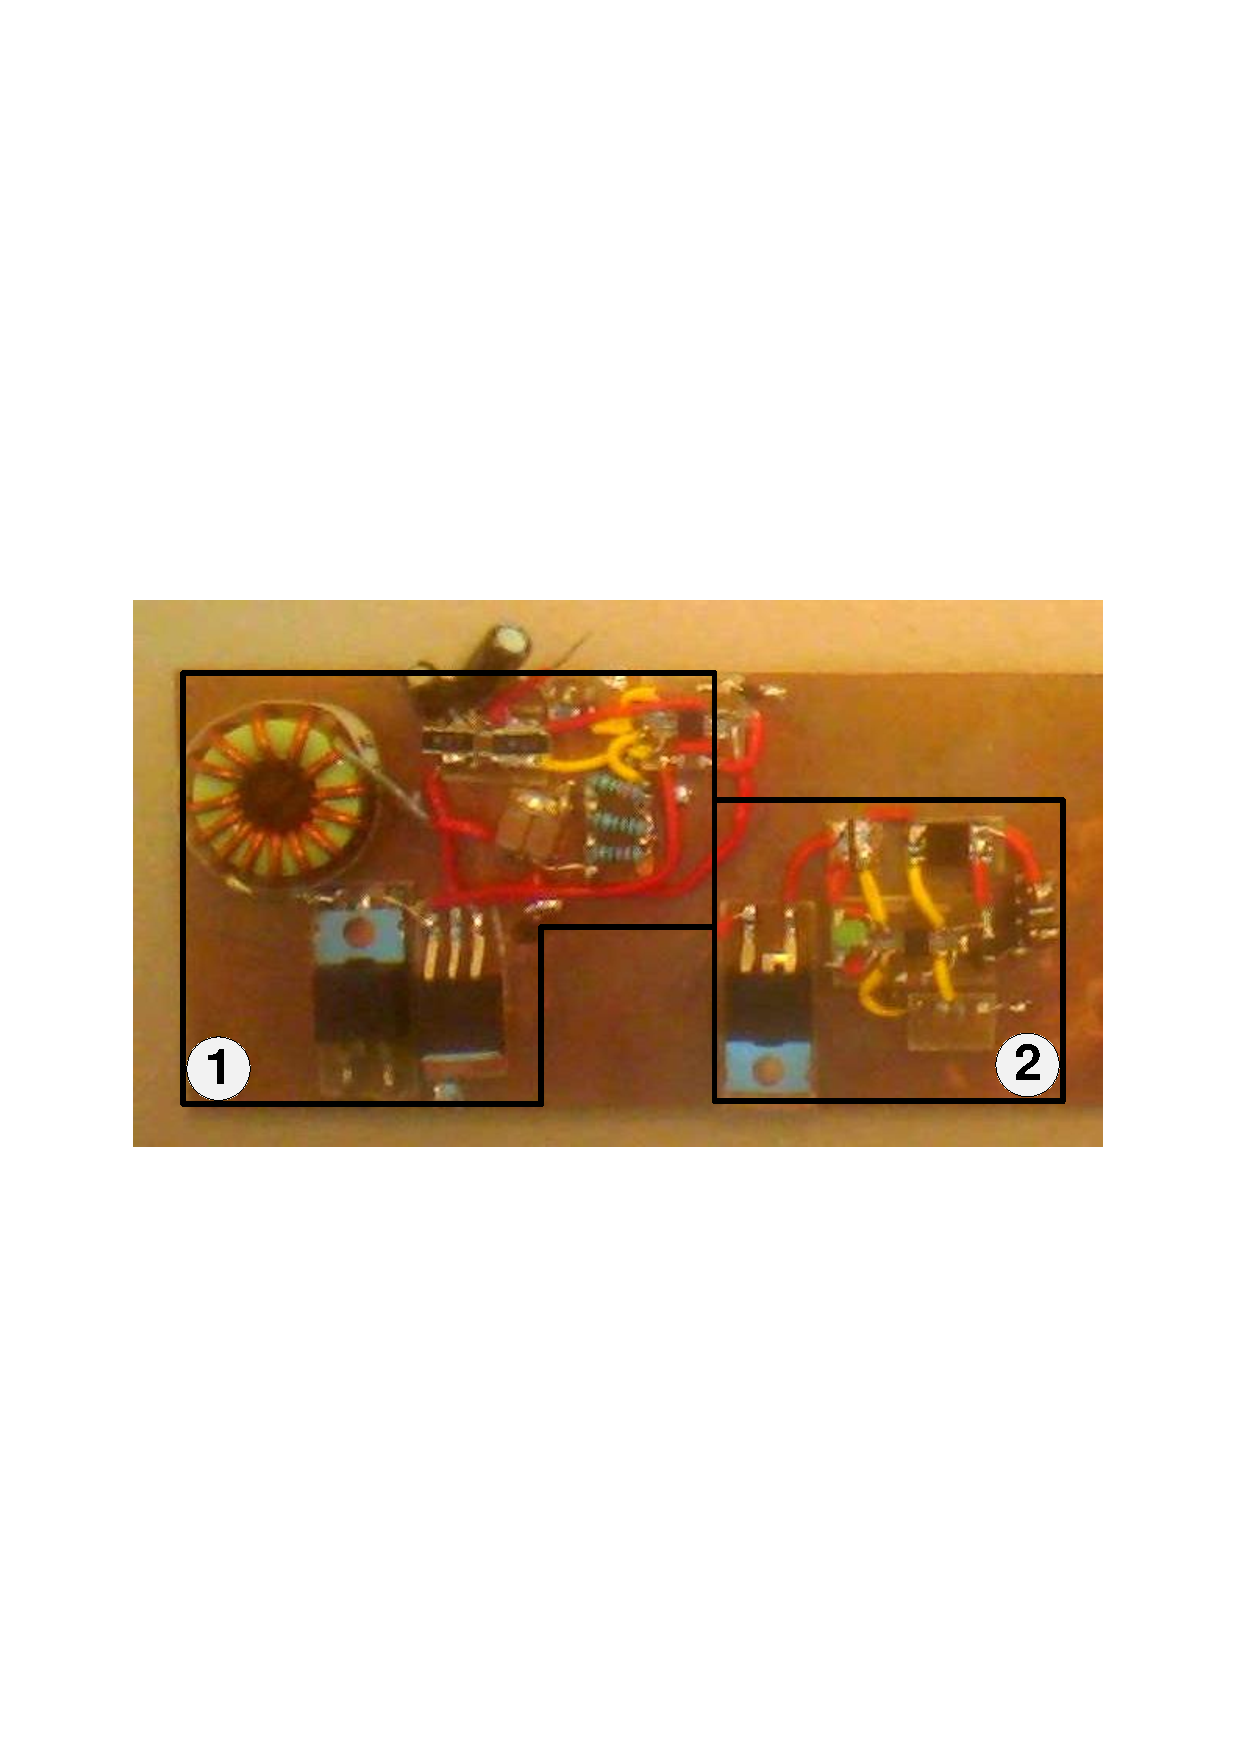
\includegraphics[width=0.8\textwidth]{figures/fig_CDR_EPSprototype}
\caption{\ac{EPS} prototype - \textbf{1}:\ac{SAR}, \textbf{2}:\ac{BCR}}
\label{fig:EPSprototype}
\end{figure}
%
\subsubsection*{Development Model Status}
The \ac{SAR} is working but shows signs of \ac{CM} instability which is expected to be caused by the missing current sense amplifier circuit and input filter. Development progress is currently awaiting delivery of components.

The \ac{BCR} is also working however excessive heating of the MOSFET was experienced. A new part rated for higher power dissipation has been selected and is currently awaiting delivery.
%
\subsubsection{EPS Flight Model}
If time allows, a dedicated \ac{FM} will be build, using a custom designed \ac{PCB} schematic layout. An optimized \ac{PCB} layout will minimize the system mass and size while maximizing the efficiency and system robustness.
%
\subsection{EPS Test Program}
Table \ref{tab:test_program} lists all necessary and desired test of the EPS. Priority "1" tests are all required while priority "2" tests will only be realized if time and resources allow it.
%
\begin{center}
\begin{longtable}[H]{p{0.15\textwidth}p{0.3\textwidth}p{0.45\textwidth}r}
\caption{EPS Test Program}\\
\label{tab:test_program}\\[-0.5cm]
\hline
\textbf{Subsystem} & \textbf{Condition/Mode} & \textbf{Test Description} & \textbf{Pri.}\\
\hline
\ac{SAR} & Mainbus voltage limitation & With more input power than load power, \ac{SAR} must be able to maintain a stable $9.5\,V$ output voltage also during transient loading & 1\\
- & Maximum power handling & With an input and load power slightly above the maximum expected solar array power, no \ac{SAR} components must overheat or otherwise malfunction & 1 \\
- & \ac{MPPT} & \ac{TBD} & 2\\
- & Mode transitions & \ac{SAR} must be able to change between \ac{MPPT}, battery charge and discharge mode without loosing mainbus voltage regulation or causing other malfunctions & 2\\
- & Feedback loop stability & Regulator bandwidth, gain- and phase margins should be measured with a Network Analyzer & 2\\
- & \ac{EMC} & Electromagnetic emissions should be measured with a Spectrum Analyzer, especially with concerns to the telecommunication systems & 2\\
\hline
\ac{BCR} & \ac{CC} and trickle charging & \ac{CC} charge at $2.4\,A$ and trickle charge mode entered when battery voltage reaches $8.4\,V$ should be verified & 1\\
- & Charge inhibit at high/low temperatures & While battery is charging, battery thermistor is heated/cooled in thermal oven/fridge to slightly above/below the specified temperature limits and charging should be terminated & 1\\
\hline
\ac{UVLO} & Power cut-off and recovery & Reducing input voltage below calculated threshold voltage should open switch and switch should close again when input voltage is increased above the threshold & 1\\
\hline
Battery & Dynamic model & Test approach is described in \cite{chen} & 2\\
\hline
Solar cell & I-V specifications & short-circuit current, open-circuit voltage, current and voltage at the \ac{MPP} should be determined from an irradiance test & 2\\
- & Temperature coefficients & Solar cell temperature coefficients should be determined be measuring the I-V characteristics at different temperatures within the expected temperature interval & 2\\
\hline
Fuses & Temperature variation & The \ac{PTC} resettable fuses should be tested at nominal, minimum and maximum expected temperatures to verify acceptable functionality & 1\\
\hline
\end{longtable}
\end{center}
%